\documentclass[../main.tex]{subfiles}

\begin{document}
Mô hình Markov ẩn (Hidden Markov Model - HMM) 

HMM là một mô hình thống kê được sử đụng dể mô tả quy trình Markov với các tham số không biết được ẩn đi. Mô hình xác định các tham số ẩn cho quy trình thông qua chuỗi các quan sát rồi sử dụng các tham số đó cho việc phân tích về sau \cite{rabiner1989tutorial}

\begin{figure}[h]
\centering
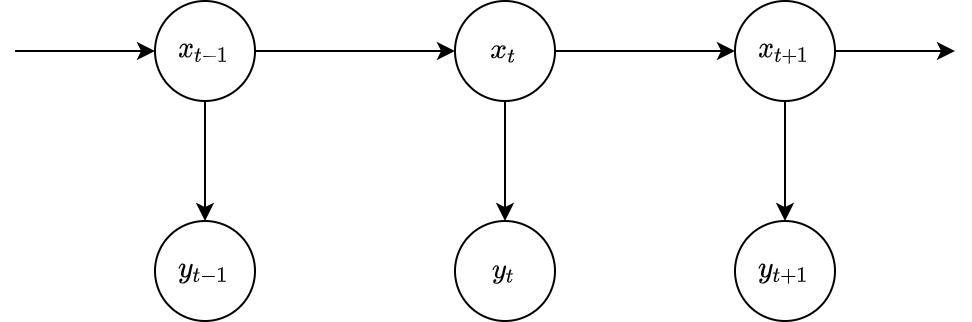
\includegraphics[scale=0.4]{02-HMM-example}
\caption{Cấu trúc của HMM}
\end{figure}

Hình 2.7 mô tả cấu trúc của HMM. $X$ là biến ẩn mà bên quan sát không phát hiện ra. $x_{t}$ biểu diễn trạng thái tại thời gian $t$. Mỗi biến quan sát được $y$ chỉ phụ thuộc vào $x_{t}$, và $x_{t}$ liên quan đến trạng thái trước đó là $x_{t-1}$

Nếu các trạng thái ẩn có $N$ giá trị, thì tại thời điểm $t$ sẽ có thể nhận N giá trị . Vì vậy, có tối đa $N^{2}$ khả năng từ một trạng thái ẩn chuyển sang trạng thái ẩn tiếp theo. Với biến quan sát $y$ có $M$ có thể nhận, mỗi giá trị trong trạng thái ẩn đều có xác suất chuyển tới tới mọi biến quan sát khác. Vì vậy, nếu chuỗi quan sát gọi là $Y$, chuỗi trạng thái ẩn là $X$, trong đó:


\begin{equation}
X = (x_{0}, x_{1}, ..., x_{n}) \nonumber
\end{equation}

\begin{equation}
Y = (y_{0}, y_{1}, ..., y_{n}) \nonumber
\end{equation}

Xác suất của chuỗi Y qua mô hình HMM có thể được biểu diễn bằng biểu thức sau: 

\begin{equation}
P(Y) = \sum_{X} P(Y|X)P(X) \nonumber
\end{equation}


Với dữ liệu chưa được gán nhãn, phương pháp thống kê của các tham số không thể tính toán được trực tiếp do sự tồn tại của các biến ẩn. Khi đó thuật toán Cực đại hóa kì vọng (Expectation Maximization - EM) được sử dụng để lặp cho đến khi hội tụ để ra được tham số cho mô hình. Thuật toán EM được chia làm $2$ phần là E và M. Ở bước E, thuật toán sử dụng tham số đã biết để tính ra hậu phân phối của biến ẩn $P(T|S, \theta^{old})$. Ở bước M, thuật toán tính giá trị kì vọng cực đại của log-likelihood dựa vào hậu phân phối. Kì vọng ở đây là một hàm có tham số $\theta$, và hàm sẽ cực đại hóa kì vọng của hàm $Q = ( \theta, \theta^{old})$ để có thể có được nghiệm của $\theta$ rồi dùng nghiệm này đưa vào $\theta^_{old}$ trong bước E. Sau đó việc này được lặp lại cho đến khi hội tụ. (\citep{zhang2001segmentation})

Sau khi quá trình huấn luyện kết thúc, sử dụng mô hình HMM có thể dự đoán chuỗi câu mới. Khi mô hình nhận vào một tập các chuỗi có được từ việc quan sát, mô hình sẽ tìm ra chuỗi ẩn phù hợp nhất sử dụng thuật toán Viterbi (\cite{ghahramani2001introduction})

Mô hình HMM đã được sử dụng rộng rãi để giải quyết nhiều bài toán về xử lý ngôn ngữ tự nhiên như nhận diện giọng nói, dịch máy, gán nhãn, nhận diện tên thực thể ... \cite{ponomareva2007biomedical}
\end{document}

